
% initial packages setting
\documentclass[12pt]{article}
\usepackage[english]{babel}
\usepackage[utf8]{inputenc}
\usepackage{fullpage}
\usepackage[usenames,dvipsnames]{xcolor}
\usepackage{amsmath}
\usepackage{amsfonts}
\usepackage{graphicx}
\usepackage{tabularx}
\usepackage{titlesec}
\usepackage{hyperref}
\hypersetup{
    colorlinks=true,
    linkcolor=black,
    filecolor=black,      
    urlcolor=black,
}

% initial cover page setting
\title{
\normalfont \normalsize 
\rule{\linewidth}{1pt} \\[10pt] 
\huge \bfseries Autonomous Drone Program Report \\
\Large \bfseries Informatics Large Practical \\
\rule{\linewidth}{1pt} \\[10pt]
}
\author{\Large \textbf{Ethan Yang}\\ \Large \textbf{s1862671}}
\date{\textbf{\today}}

% documentation begin
\begin{document}
\titleformat{\section}
{\normalfont\fontsize{16}{16}\bfseries}
{\thesection}{1em}{}
\maketitle
\newpage
\tableofcontents
\newpage
\setlength{\parindent}{0pt} % indent setting
\setlength{\parskip}{\baselineskip} % auto row space
\setlength{\parskip}{5pt}

% content begin
\section {Software Architecture Description}
\subsection {Introduction to the Autonomous Drone Program}
This section will provide overview of the autonomous drone program. The autonomous drone program is developed to collect readings from air quality sensors distributed around the University of Edinburgh’s Central Area. Drone flies around, avoids no fly zones and collects the sensor readings and produces scientific visualisations of the data in the form of GeoJSON file and produces a txt file which records flight information of drone.

\subsection {Architectural Overview of the Program}
This section will provide a comprehensive architectural overview by UML class diagram and briefly explain the purpose of each class designed and why these classes are the right ones for program. In addition, there are some explanations of advantages of this architectural design. 

\begin{center}
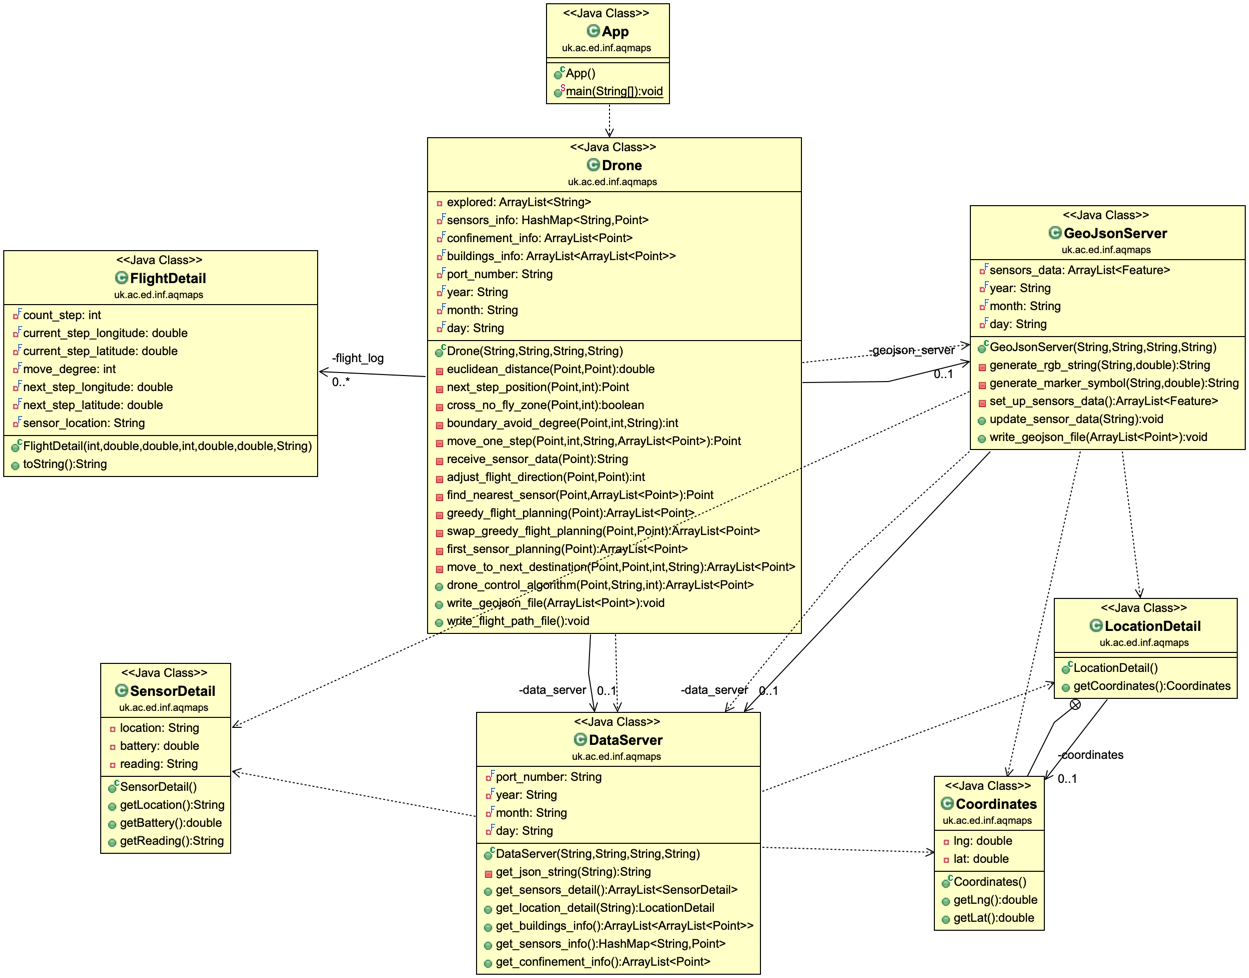
\includegraphics[width=0.95\textwidth]{UML.png}\\
\caption{Figure 1: UML Class Diagram of Program's Architecture}
\end{center}

\textbf{Class App} which is located at the top of the UML class diagram is the most significant class which contains the main method to run the program. This class only contains main method which integrates methods from Class Drone to write GeoJSON file and txt file.

\textbf{Class Drone} which is located in the middle is the biggest class and contains the most important algorithm to let drone fly around, avoid no fly zones and collect reading from sensors. This class focus on implementing drone control algorithm which is built by lots of components (small methods) and connect DataServer and GeoJsonServer which will be explained later to get data support and update sensor information to GeoJsonServer. It also write a flight path file after process of collection. This design makes Class Drone focus on single part of task without considering how to request data from web server and write GeoJSON file. 

\textbf{Class DataServer} which is located at the bottom contains all methods that get data from web server. This class only focus on parsing JSON data from web server and processing data to data structures that Class Drone need. This class also help GeoJsonServer to update information. 

\textbf{Class GeoJsonServer} which is located at the upper right focus on setting up initial state of GeoJSON map and updating information when drone receives sensor data. This class can write a GeoJSON file by using its field which stores sensors' information. 

\textbf{All these three classes are highly independent and focus on single part of tasks.} Such design has great advantages in program maintenance. If DataServer fails due to change or error occurs in web server will not affect primary design of methods in other class. Changing the format of GeoJSON file will not affect any methods designed in other class. The error that drone fails to autonomously fly around only caused by some of components of Class Drone.

\textbf{Class FlightDetail} which is located at the upper left stores all the data needed to write flight path file. Each FlightDetail object stores one row of information in flight path file which contains step number, longitude and latitude of current and next position, direction of move in degree and location of sensor detected.

\textbf{Class SensorDetail, LocationDetail and Coordinates} are used to store the data parsed from JSON file in web server. They provide common objects for three classes introduced in the last few paragraphs to store some information about sensors' data and sensors' location.

\textbf{Classes in last 2 paragraphs are just data classes.} They are designed based on format of JSON file except FlightDetail class which is designed to separate writing function from drone control algorithm. This class benefits software testing because it does not need to write txt files every time when algorithm runs in the program.

\textbf{There are some advantages of this architectural design.} Small methods divide drone control algorithm into many single functions which are easy to maintain and find bugs when program has error. Besides the refactor of program, loosely coupled design in this architecture is really important for maintenance since the web server and output requirement change over time. There is no static field which is dangerous when share address in different objects. 

\newpage
\section {Class Documentation}
\subsection {Class LocationDetail}
\textbf{Class Summary:} This class is used to provide LocationDetail object which stores location data get from web server. This class is used when store web data into its object.

\textbf{Field Detail:}

\textbf{private Coordinates coordinates} - A field refer to a Coordinates object.

\textbf{Constructor Detail}:

\textbf{public LocationDetail()} - Construct a LocationDetail object by default.

\subsection {Class Coordinates}
\textbf{Class Summary:} This class is used to provide Coordinates object which contains longitude and latitude of what3words location. This is a sub class of Class LocationDetail.

\textbf{Field Detail:}

\textbf{private double lng} - A field refer to value of longitude.\\
\textbf{private double lat} - A field refer to value of latitude.

\textbf{Constructor Detail:}

\textbf{public Coordinates()} - Construct a Coordinates object by default.

\subsection {Class SensorDetail}
\textbf{Class Summary:} This class is used to provide SensorDetail object which contains location, reading and battery value of sensor. This class is used when store web data into its object.

\textbf{Field Detail:}

\textbf{private String location} - A field refer to sensor's what3words location.\\
\textbf{private double battery} - A field refer to value of sensor battery.\\
\textbf{private String reading} - A field refer to value of sensor reading.

\textbf{Constructor Detail:}

\textbf{public SensorDetail()} - Construct a SensorDetail object by default.

\subsection {Class FlightDetail}
\textbf{Class Summary:} This class is used to provide FlightDetail object which contains all the information needed for writing flight path file by Drone.

\textbf{Field Detail:}

\textbf{private final int count\_step} - A field refer to step number of current step.\\
\textbf{private final double current\_step\_longitude} - A field refer to longitude of current step.\\
\textbf{private final double current\_step\_latitude} - A field refer to latitude of current step.\\
\textbf{private final int move\_degree} - A field refer to direction of move in degree.\\
\textbf{private final double next\_step\_longitude} - A field refer to longitude of next step.\\
\textbf{private final double next\_step\_latitude} - A field refer to latitude of next step.\\
\textbf{private final String sensor\_location} - A field refer to what3words location of sensor.

\textbf{Constructor Detail:}

\textbf{public FlightDetail(int count\_step, double current\_step\_longitude, double current\_step\_latitude, int move\_degree, double next\_step\_longitude, double next\_step\_latitude, String sensor\_location)}\\
Construct a FlightDetail object given all the information needed for flight path file.

\textbf{Method Detail:}

\textbf{public String toString()}\\
This method returns String of a row of flight path file by using fields.\\
\textbf{Returns:} String of one row of flight path file

\subsection {Class DataServer}
\textbf{Class Summary:} This class provides methods to get data from web server and provides necessary information needed for Drone to use drone control algorithm and provides necessary information needed for GeoJsonServer to write GeoJSON file.

\textbf{Field Detail:}

\textbf{private final String port\_number} - A field refer to port number of web server.\\
\textbf{private final String year} - A field refer to year of DataServer connection.\\
\textbf{private final String month} - A field refer to month of DataServer connection.\\
\textbf{private final String day} - A field refer to day of DataServer connection.

\textbf{Constructor Detail:}

\textbf{public DataServer(String year, String month, String day, String port\_number)}\\
Construct a DataServer object given date (year, month, day) and port number.

\textbf{Method Detail:}

\textbf{private String get\_json\_string(String urlString)}\\
This method connects to web server and gets JSON String from web server based on specific URL String. URL String is the address of data on web server.\\
\textbf{Parameters:} urlString - URL String\\
\textbf{Returns:} JSON String

\textbf{public ArrayList$<$SensorDetail$>$ get\_sensors\_detail()}\\
This method gets sensors' information from web server and stores in SensorDetail objects.\\
\textbf{Returns:} ArrayList of SensorDetail objects that represents sensors' information

\textbf{public LocationDetail get\_location\_detail(String W3W\_Location)}\\
This method gets what3words info from web server and stores in LocationDetail object.\\
\textbf{Parameters:} W3W\_Location - what3words location\\
\textbf{Returns:} LocationDetail object that represents what3words location

\textbf{public ArrayList$<$ArrayList$<$Point$>>$ get\_buildings\_info()}\\
This method gets no fly zones info from web server and process data into a list of list of points of no fly zones which will be used by Drone.\\
\textbf{Returns:} ArrayList of ArrayList of Point objects contains points of no fly zones

\textbf{public HashMap$<$String, Point$>$ get\_sensors\_info()}\\
This method generates a HashMap which contains 33 what3words locations of sensors as keys and corresponding points as values which will be used by Drone.\\
\textbf{Returns:} HashMap which contains what3words and location points

\textbf{public ArrayList$<$Point$>$ get\_confinement\_info()}\\
This method generates a list of corners of confinement area which will be used by Drone.\\
\textbf{Returns:} ArrayList of Point objects which contains corners of confinement area

\subsection {Class GeoJsonServer}
\textbf{Class Summary:} This class is used to provide GeoJSON service for Drone to update information received from sensors and write the GeoJSON file.

\textbf{Field Detail:}

\textbf{private final DataServer data\_server} - A field refer to DataServer object.\\
\textbf{private final ArrayList$<$Feature$>$ sensors\_data} - A field refer to sensors' data.\\
\textbf{private final String year} - A field refer to year of GeoJsonServer connection.\\
\textbf{private final String month} - A field refer to month of GeoJsonServer connection.\\
\textbf{private final String day} - A field refer to day of GeoJsonServer connection.

\textbf{Constructor Detail:}

\textbf{public GeoJsonServer(String year, String month, String day, String port\_number)}\\
Construct a GeoJsonServer object given date (year, month, day) and port number.

\textbf{Method Detail:}

\textbf{private String generate\_rgb\_string(String reading, double battery)}\\
This method converts reading to RGB String given reading and battery.\\
\textbf{Parameters:} \\
reading - value of sensor reading\\
battery - value of sensor battery\\
\textbf{Returns:} RGB String based on reading

\textbf{private String generate\_marker\_symbol(String reading, double battery)}\\
This method converts reading to marker name given reading and battery.\\
\textbf{Parameters:} \\
reading - value of sensor reading\\
battery - value of sensor battery\\
\textbf{Returns:} String of marker name based on reading

\textbf{private ArrayList$<$Feature$>$ set\_up\_sensors\_data()}\\
This method sets up field sensors\_data with default setting which contains 33 sensors' Features with no marker properties and with gray color RGB String properties.\\
\textbf{Returns:} ArrayList of Feature that represents sensors in default setting

\textbf{public void update\_sensor\_data(String location)}\\
This method updates the field sensors\_data (add properties of Feature related to what3words location parameter based on sensor reading received by Drone).\\
\textbf{Parameters:} location - what3words location

\textbf{public void write\_geojson\_file(ArrayList$<$Point$>$ points)}\\
This method writes GeoJSON file given output of drone control algorithm and sensors\_data which has been updated by drone control algorithm.\\
\textbf{Parameters:} points - ArrayList of Point that output from drone control algorithm

\subsection {Class Drone}
\textbf{Class Summary:} This class is used to provide Drone object which contains drone control algorithm and method to write flight path file and GeoJSON file.

\textbf{Field Detail:}

\textbf{private ArrayList$<$FlightDetail$>$ flight\_log}\\
list of FlightDetail objects which record flight information of Drone.\\
\textbf{private ArrayList$<$String$>$ explored} - list of what3words explored.\\
\textbf{private GeoJsonServer geojson\_server} - GeoJsonServer owned by Drone.\\
\textbf{private final DataServer data\_server} - DataServer owned by Drone.\\
\textbf{private final HashMap$<$String, Point$>$ sensors\_info}\\
33 what3words locations and corresponding points provided by DataServer.\\
\textbf{private final ArrayList$<$Point$>$ confinement\_info} - corners of confinement area.\\
\textbf{private final ArrayList$<$ArrayList$<$Point$>>$ buildings\_info} - points of no-fly zones.\\
\textbf{private final String port\_number} - port number of web server connection.\\
\textbf{private final String year} - year set by Drone.\\
\textbf{private final String month} - month set by Drone.\\
\textbf{private final String day} - day set by Drone.

\textbf{Constructor Detail:}

\textbf{public Drone(String year, String month, String day, String port\_number)}\\
Construct a Drone object given date (year, month, day) and port number.

\textbf{Method Detail:}

\textbf{private double euclidean distance(Point point1, Point point2)}\\
This method returns euclidean distance between two points.\\
\textbf{Parameters:}\\
point1 - Point object that represents a point\\
point2 - Point object that represents a point\\
\textbf{Returns:} double value that represents euclidean distance

\textbf{private Point next step position(Point current step, int degree)}\\
This method returns next point given current point and direction of move in degree.\\
\textbf{Parameters}:\\
current step - Point object that represents current point\\
degree - int value that represents direction of move in degree\\
\textbf{Returns:} Point object that represents next point

\textbf{private boolean cross\_no\_fly\_zone(Point current\_step, int degree)}\\
This method is used to determine whether current point move one step in direction of degree will intersect with boundaries of no fly zones or confinement area.\\
\textbf{Parameters:} \\
current\_step - Point object that represents current point\\
degree - int value that represents direction of move in degree\\
\textbf{Returns:} True if move one step intersect with boundaries, False otherwise

\textbf{private int boundary\_avoid\_degree(Point current\_step, int degree, String mode)}\\
This method returns direction of move in degree which avoids the boundaries of no fly zones or confinement area. Choosing the strategies to avoid boundaries based on mode.\\
\textbf{Parameters:} \\
current\_step - Point object that represents current point\\
degree - int value that represents direction of move in degree\\
mode - String that can be 'clockwise', 'anticlockwise' or 'double'\\
\textbf{Returns:} int value that represents move degree that avoids boundaries

\textbf{private Point move\_one\_step(Point current\_step, int degree, String mode, ArrayList$<$Point$>$ moved\_points)}\\
This method returns next point which avoids boundaries of no fly zones and confinement area and also make sure that next point is not in moved points.\\
\textbf{Parameters:} \\
current\_step - Point object that represents current point\\
degree - int value that represents direction of move in degree\\
mode - String that can be 'clockwise', 'anticlockwise' or 'double'\\
moved\_points - ArrayList of Point that represents moves in the past\\
\textbf{Returns:} Point object that avoids boundaries and does not occur in the past

\textbf{private String receive\_sensor\_data(Point current\_step)}\\
This method finds sensors in area of Drone detection at current point and returns the what3words location of the closest sensor.\\
\textbf{Parameters:} \\
current\_step - Point object represents current point\\
\textbf{Returns:} String that represents what3words location detected by Drone or "null"

\textbf{private int adjust\_flight\_direction(Point current\_step, Point destination)}\\
This method returns adjusted flight direction in degree which is multiple of 10.\\
\textbf{Parameters:} \\
current\_step - Point object that represents current point\\
destination - Point object that represents target sensor\\
\textbf{Returns:} int value that represents adjusted degree of move

\textbf{private Point find\_nearest\_sensor(Point sensor, ArrayList$<$Point$>$ search\_domain)}\\
This method finds the sensor that is nearest to current sensor in search domain.\\
\textbf{Parameters:} \\
sensor - Point object that represents point of current sensor\\
search\_domain - ArrayList of Point that represents unexplored sensors\\
\textbf{Returns:} Point object that represents the nearest sensor

\textbf{private ArrayList$<$Point$>$ greedy\_flight\_planning(Point first\_sensor)}\\
This method makes a flight plan of sensors based on greedy method.\\
\textbf{Parameters:} \\
first\_sensor - Point object that represents position of first sensor\\
\textbf{Returns:} ArrayList of Point that represents list of sensors to be visited by order

\textbf{private ArrayList$<$Point$>$ swap\_greedy\_flight\_planning(Point start\_position, Point first\_sensor)}\\
This method makes a flight plan of sensors based on greedy method with swap heuristic.\\
\textbf{Parameters:} \\
start\_position - Point object that represents start position of Drone\\
first\_sensor - Point object that represents position of first sensor\\
\textbf{Returns:} ArrayList of Point that represents list of sensors to be visited by order

\textbf{private ArrayList$<$Point$>$ first\_sensor\_planning(Point start\_position)}\\
This method returns an ArrayList of sensors from closest to furthest given drone position.\\
\textbf{Parameters:} \\
start\_position - Point object that represents start position of Drone\\
\textbf{Returns:} ArrayList of Point that represents list of sensors from closest to furthest

\textbf{private ArrayList$<$Point$>$ move\_to\_next\_destination(Point current\_step, Point destination, int count\_steps, String mode)}\\
This method controls the Drone move from current position to target sensor.\\
\textbf{Parameters:} \\
current\_step - Point object that represents current position\\
destination - Point object that represents next sensor to detect\\
count\_steps - int value that represents current step number\\
mode - String that can be 'clockwise', 'anticlockwise' or 'double'\\
\textbf{Returns:} ArrayList of Point that contains all points in process of move

\textbf{public ArrayList$<$Point$>$ drone\_control\_algorithm(Point start\_position, String mode, int tolerant)}\\
This method controls Drone to collect data from sensors following plan made by planning algorithm.\\
\textbf{Parameters:} \\
start\_position - Point object represents start position of Drone\\
mode - String that can be 'clockwise', 'anticlockwise' or 'double'\\
tolerant - int value that represents max times of replanning.\\  
\textbf{Returns:} ArrayList of Point that contains all points of move during process

\textbf{public void write\_geojson\_file(ArrayList$<$Point$>$ path)}\\
This method writes GeoJSON file by GeoJsonServer's method given flight path of Drone.\\
\textbf{Parameters:} \\
path - ArrayList of Point that contains points of move in whole flight process

\textbf{public void write\_flight\_path\_file()}\\
This method writes flight path file by using field flight\_log.

\subsection {Class App}
\textbf{Class Summary:} This class is used to provide the main method which integrates methods from Drone to write both GeoJSON file and flight path file based on command line inputs.

\textbf{Method Detail:}

\textbf{public static void main(String[] args)}\\
This methods writes GeoJSON file and txt file by choosing one output of drone control algorithm that has minimum number of steps among three different mode. All parameters come from command line.\\
\textbf{Command Line Input:}\\
day month year latitude longitude seed port\_number\\
where latitude and longitude are drone start position.

\newpage
\section {Drone Control Algorithm}
\subsection {Introduction to the Algorithm}

This section will introduce the whole drone flight process in detail. And in next few sections, there are comprehensive explanations of essential algorithms used during process. The general idea of drone control algorithm is really simple. Drone firstly makes a plan to decide what order of sensors that it will go to collect data and then follows the plan and flies directly towards those sensors one by one until all the sensors' data have been collected and finally return to the start position. During the process, it will avoid all the no fly zones between one sensor and another sensor, so it will change the direction of move if next move of drone will hit the no fly zones. This general process has been shown in the figure below which is produced by geojson.io:
\begin{center}
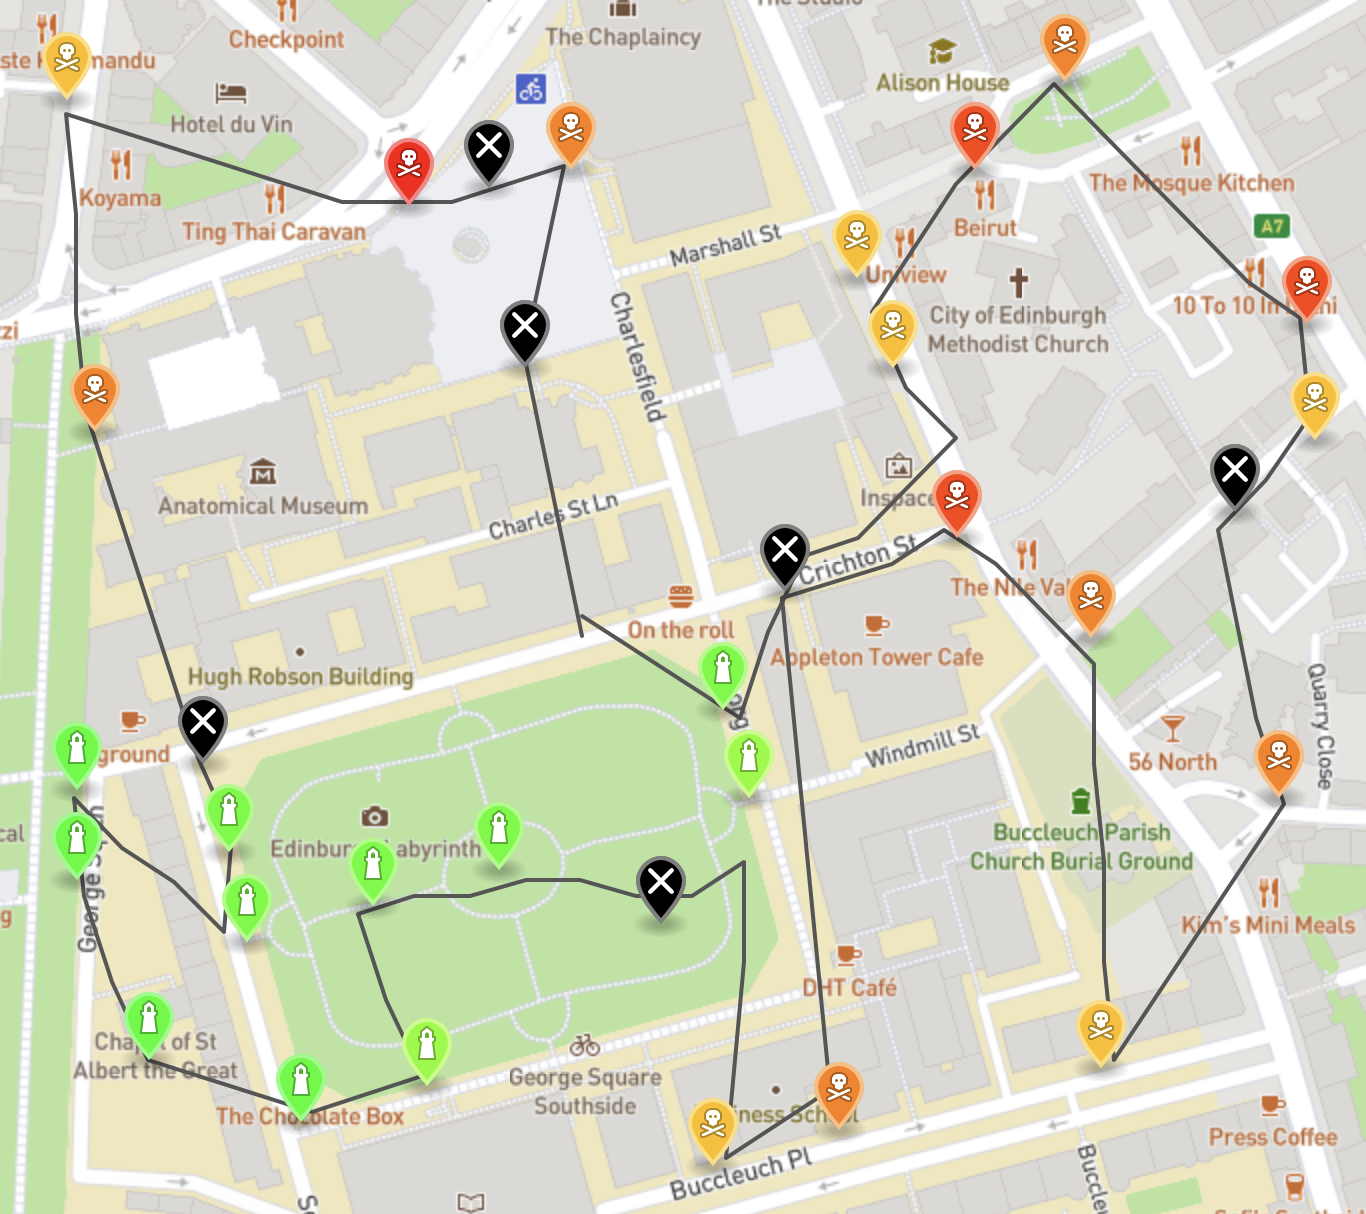
\includegraphics[width=0.83\textwidth]{2020-08-08.png}\\
\caption{Figure 2: A sample output map for the date 08/08/2020.}
\end{center}
From figure above, we can see that the drone starts at central area of the university and go to each sensors step by step, while avoiding no fly zones. It is clear to see that drone cross narrow street between Informatics Forum and Appleton Tower which are two no fly zones commonly between one sensor and another sensor. Drone collects sensor's data within 0.0002 degree of sensor so some parts of path are not close enough to sensors. Overall, the drone use a reasonably good strategy to plan the order of sensors so that the flight path is really efficient.

\subsection {No-fly Zone Avoidance Algorithm}
This section will explain no-fly zone avoidance algorithm which play a significant role in the drone control algorithm. The figure in last section has shown how this algorithm avoids no fly zones and in this section, it will be explained in detail. This algorithm has been implemented in \textbf{cross\_no\_fly\_zone}, \textbf{boundary\_avoid\_degree} and \textbf{move\_one\_step} methods in \textbf{Class Drone}. The general idea of algorithm is that if the flight path between current position and next position of drone in one move intersects with any boundaries of no fly zones, the drone can be considered as 'hit the no fly zones'. 

When drone hits the no fly zones, the drone has three different strategies to solve the problem. The choice of strategies is based on 'mode' parameter. There are three values for 'mode' parameter - 'clockwise', 'anticlockwise' and 'double'. 'clockwise' is a strategy that turns the degree of move which towards target sensor in clockwise direction until next position will not hit the no fly zones. In similar way, 'anticlockwise' is a strategy in the same way but turns degree in anticlockwise direction. 'double' is more smart than those two and will determine which direction will turn less degree to avoid hitting no fly zones. The drone uses those three strategies and a consistent rule that in every steps, drone will towards the target sensor that it want to collect data. This makes flight path of drone similar to fly along the edge of no fly zones which is shown in figure 2. This algorithm still make sure that if drone does not hit no fly zones, it will move towards target sensor directly. 

If you think about algorithm rigorously, you will find bugs in these strategies. For examples, if the edge of no fly zones is too long, the 'double' will fail by moving left and right repeatedly and finally get stuck. There is a solution given in this algorithm. If next position of drone is where has been reached in the past, the drone will change the degree to opposite direction of that degree and find an appropriate degree which will not hit no fly zones. This helps 'double' get out of local trap. Overall, this algorithm is really robust to avoid no fly zones although sometimes drone will move strangely when it meets groove. 

\subsection {Swap Greedy Path Planning Algorithm}

This section will explain swap greedy path planning algorithm which helps drone to make a wise choice to plan the order of sensors. This algorithm is implemented in two methods \textbf{find\_nearest\_sensor} and \textbf{swap\_greedy\_flight\_planning} in \textbf{Class Drone}. In figure 3, we can see that most of time the drone will choose the closest sensor to visit and this process will repeat over and over again until all the sensors has been visited. This is the idea of greedy part of algorithm. However, greedy algorithm has a limitation that it is easy to get local optimal results rather than global optimal result. The pure greedy algorithm sometimes can not get efficient plan since plan is based on straight line approximation without considering the real situation such as avoiding no fly zones. 
\begin{center}
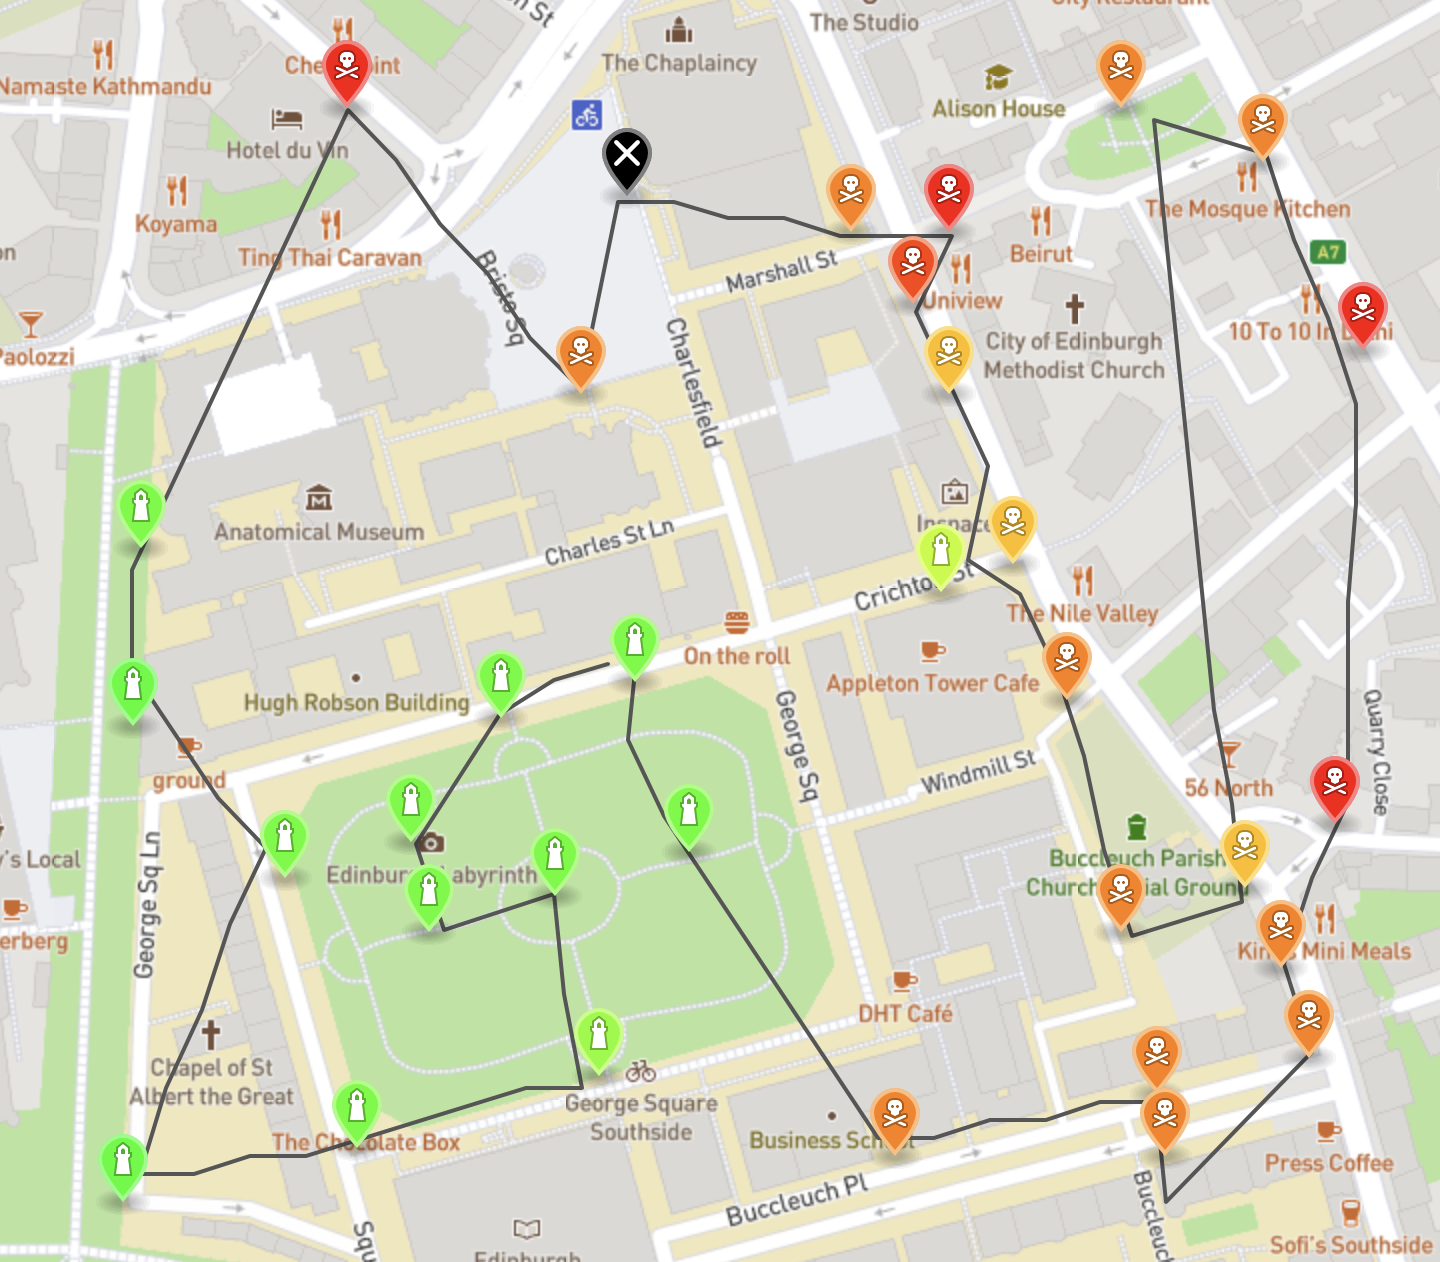
\includegraphics[width=0.83\textwidth]{2020-01-01.png}\\
\caption{Figure 3: A sample output map for the date 01/01/2020.}
\end{center}
There is an improvement for greedy algorithm called swap heuristic. The general idea of swap heuristic is that swapping two sensors in a list when total distance of sensors decreases after swapping. This process will repeat until all possible swaps in this list has been tried. This is swap part of algorithm. There is also a heuristic part. If swap occurs in the whole tries, the whole tries will start again until there is no any swap occurs in the whole tries. Swap greedy path planning algorithm combines both greedy algorithm and swap heuristic. The algorithm will firstly use greedy to get a intuitively good plan and then use swap heuristic to help greedy get out of local optimal. Swap greedy algorithm always give a circular path which hardly ever has intersecting lines in flight path. This has been shown in upper right of figure 3 where drone decides to go to a furthest sensor below rather than nearest red sensor and then visits a list of sensors which are close to each other from below to above. Swap Heuristic unties the intersecting lines made by greedy and shorten the path.

\subsection {Path Re-Planning Algorithm}
This section will explain path re-planning algorithm which is hardly ever used in drone control algorithm but plays a significant role when it is necessary. This algorithm is implemented in \textbf{first\_sensor\_planning} and \textbf{drone\_control\_algorithm} in \textbf{Class Drone}. If you think about the algorithms shown in last few sections, there is a risk that drone possibly flight around in a groove and wast a lot of steps to get out of groove and finally cannot finish collection within 150 steps. And in extreme situation, it is possible that drone still get stuck in local trap. Although those situation is rare, algorithm failure still need to be considered.

One way to solve this problem is re-planning the flight path which changes the first sensor planned by swap greedy path planning algorithm. Greedy algorithm is sensitive to choice of first sensor due to its local optimal drawback. This drawback can be used as a way to re-plan the flight path by trying different sensors as first sensor. The order to try different sensors should be intuitive. So algorithm sorts all sensors by distance between sensors and drone start position from closest to furthest and use this order to try re-planning. This algorithm has a parameter 'tolerant' which can be set to any integer value between 1 and 33. This parameter can decides how many algorithm failure can be tolerated. Over this value, the algorithm will stop regardless it success or not. This parameter design is due to Java memory limit and thread limit.

\subsection{Path Minimization Algorithm}
This section will explain last algorithm in drone control algorithm which is implemented in \textbf{main method} of \textbf{Class App}. This algorithm uses three different modes introduced in no fly zones avoidance algorithm and get three different results. After that choosing one which has minimum steps among three modes and writing flight path file and GeoJSON file based on it. This algorithm helps drone to choose a more efficient flight path and largely decrease the risk of algorithm failure.

\section{References}
\href{https://docs.mapbox.com/android/java/overview/}{Third party library Mapbox Java SDK is used in program - click here}\\
\href{http://www.jibble.org/jibblewebserver.php}{Jibble Web Server - Web Server used in program - click here}\\
\href{https://en.wikipedia.org/wiki/Travelling\_salesman\_problem#Heuristic\_and\_approximation\_algorithms}{Swap and Greedy Heuristic - Travelling salesman problem in Wikipedia - click here}\\
\href{https://en.wikipedia.org/wiki/Greedy_algorithm}{Greedy Algorithm - Introduction in Wikipedia - click here}\\
\href{https://en.wikipedia.org/wiki/2-opt}{Two Opt Swap Algorithm - Introduction in Wikipedia - click here}\\
All other algorithms are self designed without references

\section{Appendices}

\end{document}